\graphicspath{ {Chapters/images/} }
\chapter{Material and Methods}
\section{Overview}

The simulation data sets used Escherichia coli K12 as the reference genome. The donor genome is simulated by randomly placing different sizes of insertions and deletions. Paired-end and mate-pair reads were randomly sheared from the donor genome with coverage 25x via Wgsim from the SAMtools package. The two real data sets are Illumina sequencing data from two rice species (called TN67 and Shio). Both TN67 and Shio have pair-end sequencing with coverage 30x and mate pair sequencing with coverage 100x. The rice reference genome (O. Sativa) is downloaded from the MSU rice genome annotation project.

Our method aims to reconstruct the donor genome by a closely-related reference genome. Potential insertions and deletions (between the reference and donor genomes) are detected using signatures in alignment results of paired-end reads and mate pair reads. Secondly, we assemble detected insertion sequences using a contig graph constructed from paired end reads, and place the insertion or remove deletions from the reference genome to generate a draft genome. Finally, the assembled contigs from paired end reads is used to replace SNPs and indels to reconstruct the donor genome. Figure 3.1 illustrated the flowchart of our method.

\begin{figure}[ht]
\begin{center}
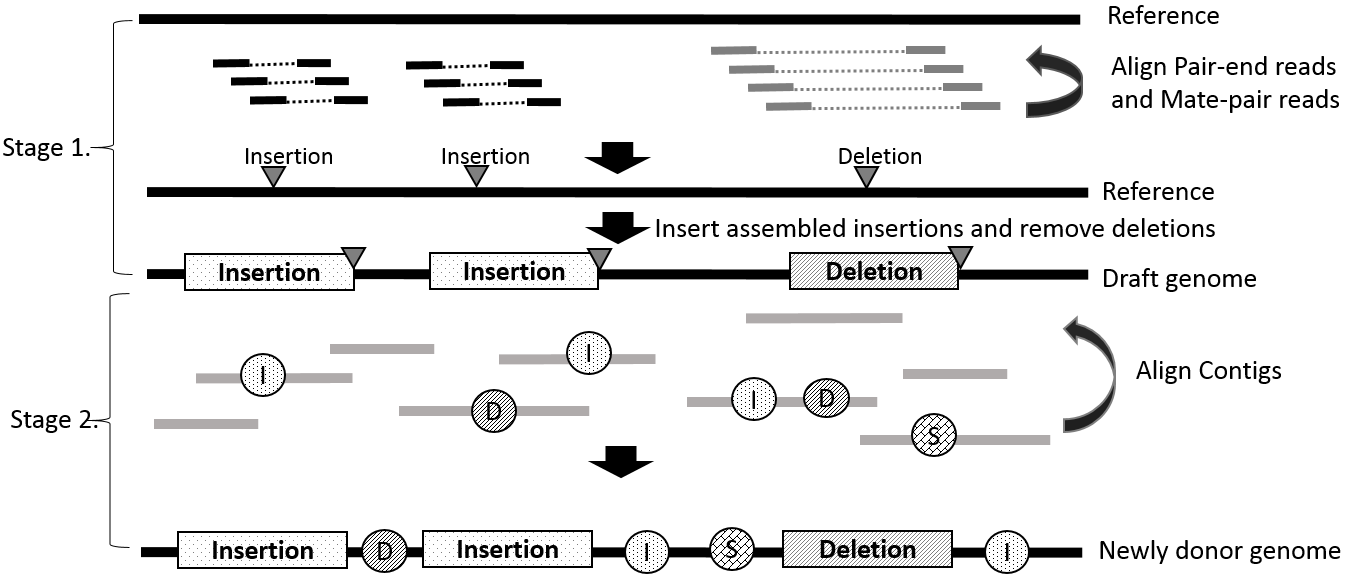
\includegraphics[scale=0.4]{workflow}
\caption{Overview of our method. Stage1: Inserting assembled large-sized insertions and removing deletions to reconstruct a draft genome. Stage2: The draft genome sequence is replaced with the contig sequences, which is able to reflect inter-species SNPs and small-sized indels. Finally, we can get a newly donor genome with large-sized insertions/deletions, small-sized indels, and inter-species SNPs.   }
\label{}
\end{center}
\end{figure}

\newpage
\section{Detection of Potential Insertions and Deletions}

At first, paired-end reads and mate-pair reads of the donor genome separately align onto the closely-related genome via BWA~\cite{BWA}. Several signatures of insertions and deletions can be found in the SAM alignment, including breakpoint reads and aberrant mapping distances (Figure 3.2). 

\begin{figure}[ht]
\begin{center}
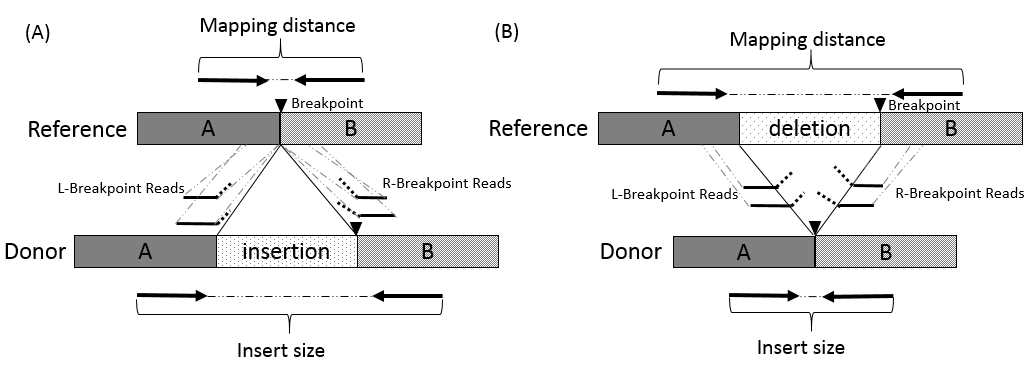
\includegraphics[scale=0.5]{break_signature}
\caption{Paired end reads are aligned to the reference genome. If there exists an insertion or deletion in the donor genome, local alignment of reads nearby the breakpoint are called breakpoint reads. Solid part of breakpoint reads means mapped sequence, and the dashed part of breakpoint reads means unmapped sequence. (A)Insertion. (B)Deletion.}
\label{}
\end{center}
\end{figure}

\subsection{Signatures of Breakpoint Reads}

The breakpoint reads (also called split reads) are reads that span the insertion or deletion loci, and the alignment results of these reads onto a reference often lead to partial local alignments. We further distinguish left and right breakpoint reads according to the position of local alignment with respect to the left or right of the locus. The numbers of left and right breakpoints are defined as $n_l$ and $n_r$.

In practice, owing to repeats, chimera reads, and alignment errors, not all these breakpoint reads are indicative of insertions and deletions. For instance, the numbers of loci containing breakpoint reads can be up to 2,476,410 in the rice genomes. The threshold of minimum $n_l$ and $n_r$ required to call an insertion or deletion is also related to the sequencing coverage. In order to uncover the relation between the threshold and coverage, a number of simulation data sets with different sequencing coverage are conducted. We collected minimum $n_l$ and $n_r$ to estimate the number of breakpoint reads. Linear regression was used to infer the relation between the number of breakpoints $T$ and the sequencing coverage $C$, which is.
\begin{equation} T=1+0.08C
\end{equation}
Since the sequencing coverage $C$ is always known in advance, we can determine the threshold $T$ accordingly. We determine there may be an insertion or a deletion by both the number of left breakpoint reads and the number of right breakpoint reads are larger then $T$. 
\begin{figure}[ht]
\begin{center}
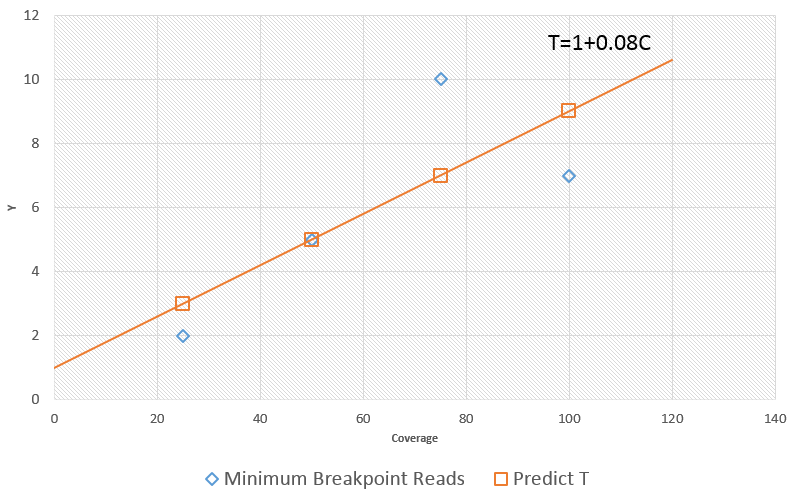
\includegraphics[scale=0.5]{regression}
\caption{A tendency chart about expected T at different coverages.}
\label{}
\end{center}
\end{figure}







\subsection{Signatures of Aberrant Mapping Distance}

Another signature of an insertion or a deletion is aberrant mapping distance between two ends of a read which deviates from the expected distance ($d_e$). By aligning mate pair reads on to the reference genome, an insertion can be detected if mapping distance is smaller than expected insert size. Conversely, if there is a deletion in the donor genome, the mapping distance is larger than expected insert size. For each breakpoint, we collect the mapping distances of mate pair reads with two ends across each breakpoint $b_i$. The median of mapping distances across each breakpoint is defined as ($d_{b_i}$) (see Figure 3.3). 


\begin{figure}[ht]
\begin{center}
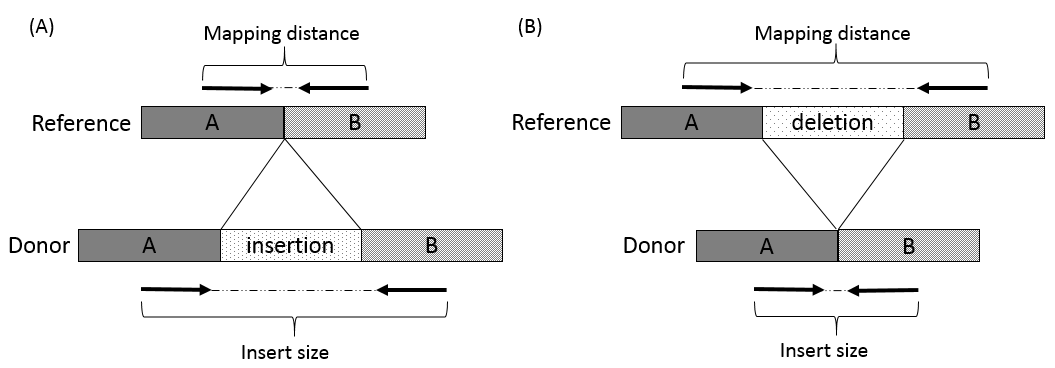
\includegraphics[scale=0.5]{mapping}
\caption{Mate pair reads are aligned to the reference genome.(A)If there is an insertion in the donor genome, mapping distance is smaller than the insert size; (B)If there is a deletion in the donor genome, mapping distance is larger than the insert size.   }
\label{}
\end{center}
\end{figure}


\subsection{Identification of Insertions and Deletions}

    In practice, we first identify all the genomic loci with $n_r > T$. Note that we can't know if each locus is insertion or deletion at this moment. Subsequently, the median of mapping distance $d_{b_i}$ is computed and compared against $d_e$. This position is considered as insertion if $d_{b_i}<d_e$. Otherwise ($d_{b_i}>d_e$), it is considered as deletion.  

    Furthermore, the number of reads fully aligned across the breakpoint ($nf_{b_i}$) should be as few as possible. And the left breakpoint reads $n_l$ should be greater than $T$. In summary, an insertion or deletion is called if satisfying all the following rules: (1) $nl_{b_i} > T$ and $nr_{b_i} > T$, (2) $nf_{b_i}$, and (3) $d_{b_i} < d_e$. 

    The length of insertions is estimated by $D_e$ minus $D_m$. Although deletions can be estimated in similar way, it can be precisely computed by the distance between the left and right breakpoint loci, which are exactly the same as the deletion size (see Figure 3.4). 


\begin{figure}[ht]
\begin{center}
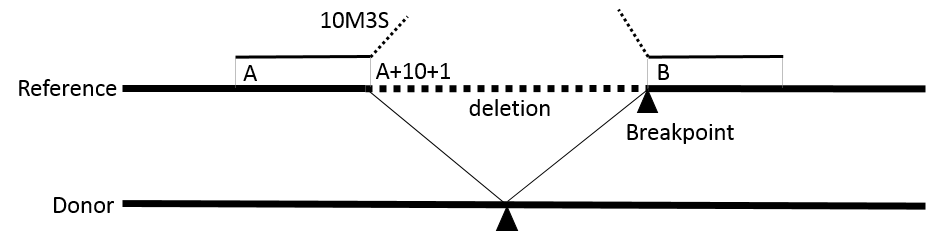
\includegraphics[scale=0.5]{Deletion_range}
\caption{ A left breakpoint read which CIGAR is 10M3S at position A, and the breakpoint at position B. The range of the deletion is A+10+1 to B-1. }
\label{}
\end{center}
\end{figure}

\newpage
\section{Assembly of Insertion Sequences}

Although the insertion loci can be inferred using the above method, the insertion sequences are not reconstructed. In order to assemble these insertion sequences, we solve a local assembly problem using a contig graph generated by SGA. The first step aims to map the left/right sequences flanking each insertion onto vertices in the graph. The second step aims to reconstruct the insertion sequence from contig graph.

\subsection{Mapping of Insertion Flanking Sequences onto Contig Graph}

Paired-end reads are assembled to contigs by SGA, which outputs a contig sequences and a contig graph (Figure 3.5). Subsequently, we extract one left and one right sequences flanking each insertion locus (called L-Read and R-Read), and map the two sequences onto the contig graph via the following procedure. 

The mapping procedure relies on an FM-index constructed from contig sequences (assembled by SGA~\cite{Simpson2012a}). Each pair of L-Read and R-Read are mapped onto the contig sequences (containing them as substrings) using the backward-search algorithm~\cite{Ferragina2000}. 

If both L-Read and R-Read are mapped onto same vertex in the contig graph, the sequence of the insertion is return. Otherwise, we try to find paths between the two vertices that L-Read mapped (called start vertex) and the contig that L-Read mapped (called end vertex) on the contig graph. By performing breadth-first search of contigs, we reconstruct the sequence of insertions.



\begin{figure}[ht]
\begin{center}
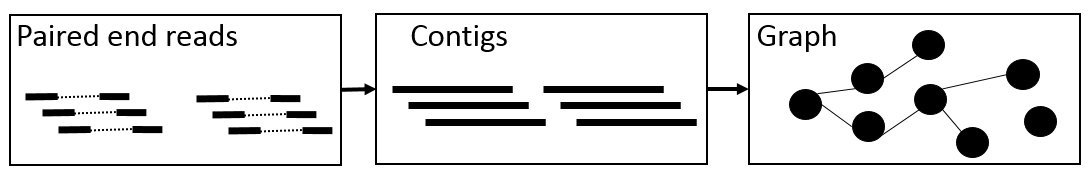
\includegraphics[scale=0.5]{contig_graph}
\caption{Paired-end reads are assembled to contigs. And then, using these assembled contigs to construct a contig graph.}
\label{}
\end{center}
\end{figure}

\begin{figure}[ht]
\begin{center}
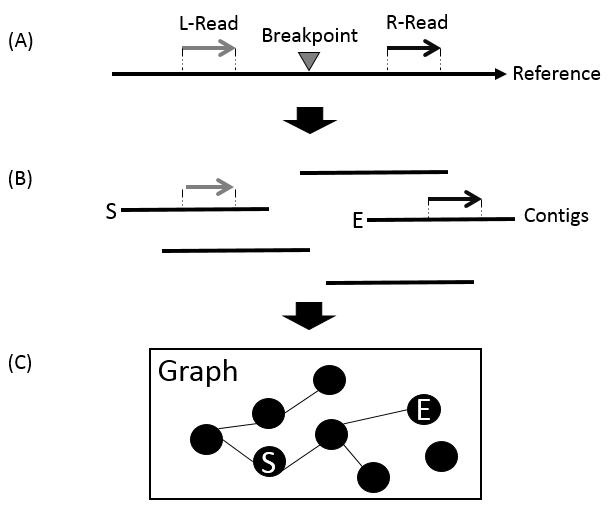
\includegraphics[scale=0.5]{align_readtocontig}
\caption{}
\label{}
\end{center}
\end{figure}

\newpage

\subsection{Breadth First Search of Insertion Sequence}

Given a start vertex and an end vertex on the contig graph, we use the algorithm findwalks of SGA to search paths between start contig and end contig. Assembly is performed by traversing the contig graph in a breadth-first search order from a given start vertex. The process stop while the maximum distance (set to sum of predict length, start vertex size and end vertex size) between the start vertex and the end vertex is reached, or the maximum number of leaves (set to 3000k) is reached. 

When traversing the contig graph, it records the paths while the expended node is the end vertex. Get the sequences from all recorded paths present, we select one of these sequence which length is closest to the predict length of the insertion. And then,we can return the sequence as insertion sequence. It means that the absolute value of the predict length minus path length is minimum. 

By using predict length of insertion, we will find the more correct path from all possible paths. For example, if the insertion contains two repeats, it may construct a path containing one repeat and a path containing two repeats. As the result, the predict length is helpful for selecting the path containing two repeats(See Figure 3.7). If no path that can reach end vertex from start vertex, the insertion is assembled unsuccessfully. 




\begin{figure}[ht]
\begin{center}
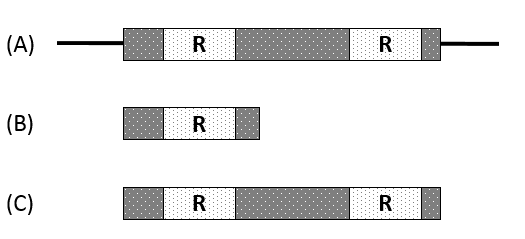
\includegraphics[scale=0.5]{repeat_insertion}
\caption{(A) is the real insertion contains repeats R. (B) and (C) are two assembled insertions from two possible paths. Using predict length of insertion, we can select (C) not (B).  }
\label{}
\end{center}
\end{figure}

\section{Alignment of Contigs to the Draft Genome}

We can generate a draft genome after placing large-sized insertions and removing deletions from the reference genome. Although we can detect and assemble large-sized insertions and range of deletions, there are SNPs and small indels between the donor genome and the closely-related reference genome. SNPs and indels are easy to construct by assembling reads to contigs because they could be generated into assembled contigs. So, we align assembled contigs onto the draft genome. SNPs and indels will be filled into the draft genome with the aligned portions of these contigs by parsing the SAM alignment results.

At first, the SAM alignment results are sorted by the alignment positions. And then, we substitute the aligned portion of the contig for draft genome while the end position of the aligned portion of the contig is larger than previous contig, conversely, we skip this alignment result. Figure3.8 illustrate the way to substitute the aligned portion by aligned contigs.
Finally, the draft genome sequence is replaced with the contig sequences, which is able to reflect inter-species SNPs and small-sized indels.

\begin{figure}[ht]
\begin{center}
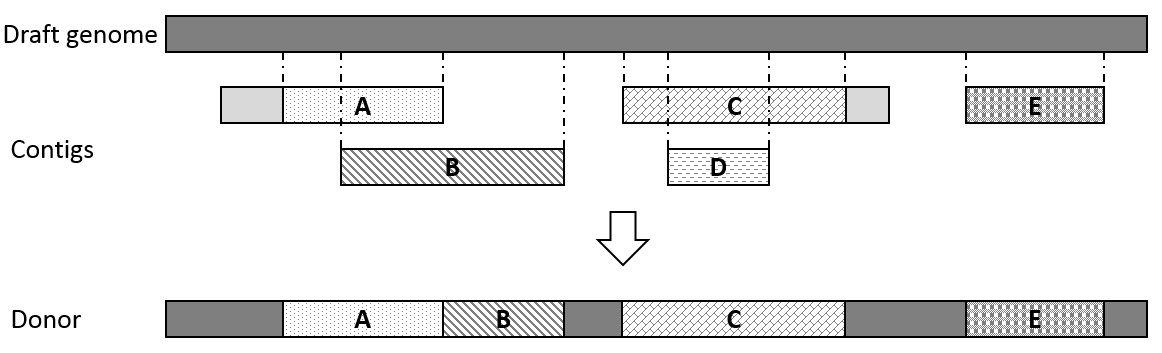
\includegraphics[scale=0.4]{contig_align}
\caption{The SAM alignment results of contigs are sorted with the alignment position. The dash lines show the aligned portion of each contig. At first, we substitute the aligned portion of contig A for the aligned portion of reference genome. Secondly, we substitute partly aligned portion of contig B for the aligned portion of the reference genome because the start aligned position of contig B is smaller than the end aligned position of contig A. And then, we process contig C and E. The result of skipping contig D is that the end aligned position of contig D is smaller than the end aligned position of contig C. Finally, we get a newly donor genome after all the contigs are done.}
\label{}
\end{center}
\end{figure}

















